% THIS DOCUMENT IS TAILORED TO REQUIREMENTS FOR SCIENTIFIC COMPUTING.  IT SHOULDN'T
% BE USED FOR NON-SCIENTIFIC COMPUTING PROJECTS
\documentclass[12pt]{article}

\usepackage{amsmath, mathtools}
\usepackage{amsfonts}
\usepackage{amssymb}
\usepackage{graphicx}
\usepackage{colortbl}
\usepackage{xr}
\usepackage{hyperref}
\usepackage{longtable}
\usepackage{xfrac}
\usepackage{tabularx}
\usepackage{float}
\usepackage{siunitx}
\usepackage{booktabs}
\usepackage{caption}
\usepackage{pdflscape}
\usepackage{afterpage}

\usepackage[round]{natbib}

%\usepackage{refcheck}

\hypersetup{
    bookmarks=true,         % show bookmarks bar?
      colorlinks=true,       % false: boxed links; true: colored links
    linkcolor=red,          % color of internal links (change box color with linkbordercolor)
    citecolor=green,        % color of links to bibliography
    filecolor=magenta,      % color of file links
    urlcolor=cyan           % color of external links
}

%% Comments

\usepackage{color}

\newif\ifcomments\commentstrue %displays comments
%\newif\ifcomments\commentsfalse %so that comments do not display

\ifcomments
\newcommand{\authornote}[3]{\textcolor{#1}{[#3 ---#2]}}
\newcommand{\todo}[1]{\textcolor{red}{[TODO: #1]}}
\else
\newcommand{\authornote}[3]{}
\newcommand{\todo}[1]{}
\fi

\newcommand{\wss}[1]{\authornote{blue}{SS}{#1}} 
\newcommand{\plt}[1]{\authornote{magenta}{TPLT}{#1}} %For explanation of the template
\newcommand{\an}[1]{\authornote{cyan}{Author}{#1}}

%% Common Parts

\newcommand{\progname}{Damped Harmonic Ocsillator} % PUT YOUR PROGRAM NAME HERE
\newcommand{\authname}{
\\ Muhammad Waqar Ul Hassan Awan
} % AUTHOR NAMES                  

\usepackage{hyperref}
    \hypersetup{colorlinks=true, linkcolor=blue, citecolor=blue, filecolor=blue,
                urlcolor=blue, unicode=false}
    \urlstyle{same}
                                


% For easy change of table widths
\newcommand{\colZwidth}{1.0\textwidth}
\newcommand{\colAwidth}{0.13\textwidth}
\newcommand{\colBwidth}{0.82\textwidth}
\newcommand{\colCwidth}{0.1\textwidth}
\newcommand{\colDwidth}{0.05\textwidth}
\newcommand{\colEwidth}{0.8\textwidth}
\newcommand{\colFwidth}{0.17\textwidth}
\newcommand{\colGwidth}{0.5\textwidth}
\newcommand{\colHwidth}{0.28\textwidth}

% Used so that cross-references have a meaningful prefix
\newcounter{defnum} %Definition Number
\newcommand{\dthedefnum}{GD\thedefnum}
\newcommand{\dref}[1]{GD\ref{#1}}
\newcounter{datadefnum} %Datadefinition Number
\newcommand{\ddthedatadefnum}{DD\thedatadefnum}
\newcommand{\ddref}[1]{DD\ref{#1}}
\newcounter{theorynum} %Theory Number
\newcommand{\tthetheorynum}{TM\thetheorynum}
\newcommand{\tref}[1]{TM\ref{#1}}
\newcounter{tablenum} %Table Number
\newcommand{\tbthetablenum}{TB\thetablenum}
\newcommand{\tbref}[1]{TB\ref{#1}}
\newcounter{assumpnum} %Assumption Number
\newcommand{\atheassumpnum}{A\theassumpnum}
\newcommand{\aref}[1]{A\ref{#1}}
\newcounter{goalnum} %Goal Number
\newcommand{\gthegoalnum}{GS\thegoalnum}
\newcommand{\gsref}[1]{GS\ref{#1}}
\newcounter{instnum} %Instance Number
\newcommand{\itheinstnum}{IM\theinstnum}
\newcommand{\iref}[1]{IM\ref{#1}}
\newcounter{reqnum} %Requirement Number
\newcommand{\rthereqnum}{R\thereqnum}
\newcommand{\rref}[1]{R\ref{#1}}
\newcounter{nfrnum} %NFR Number
\newcommand{\rthenfrnum}{NFR\thenfrnum}
\newcommand{\nfrref}[1]{NFR\ref{#1}}
\newcounter{lcnum} %Likely change number
\newcommand{\lthelcnum}{LC\thelcnum}
\newcommand{\lcref}[1]{LC\ref{#1}}

\usepackage{fullpage}

\newcommand{\deftheory}[9][Not Applicable]
{
\newpage
\noindent \rule{\textwidth}{0.5mm}

\paragraph{RefName: } \textbf{#2} \phantomsection 
\label{#2}

\paragraph{Label:} #3

\noindent \rule{\textwidth}{0.5mm}

\paragraph{Equation:}

#4

\paragraph{Description:}

#5

\paragraph{Notes:}

#6

\paragraph{Source:}

#7

\paragraph{Ref.\ By:}

#8

\paragraph{Preconditions for \hyperref[#2]{#2}:}
\label{#2_precond}

#9

\paragraph{Derivation for \hyperref[#2]{#2}:}
\label{#2_deriv}

#1

\noindent \rule{\textwidth}{0.5mm}

}

\begin{document}

\title{Software Requirements Specification for \progname:
Damped Harmonic Oscillator Illustrated by Online Calculator} 
\author{\authname}
\date{\today}
	
\maketitle

~\newpage

\pagenumbering{roman}

\tableofcontents

~\newpage

\section*{Revision History}

\begin{tabularx}{\textwidth}{p{3cm}p{2cm}X}
\toprule {\bf Date} & {\bf Version} & {\bf Notes}\\
\midrule
February 2, 2024 & 1.0 & Initial Document Release\\
\bottomrule
\end{tabularx}

~\newpage

\section{Reference Material}

This section records information for easy reference.

\subsection{Table of Units}

Throughout this document SI (Syst\`{e}me International d'Unit\'{e}s) is employed
as the unit system.  In addition to the basic units, several derived units are
used as described below.  For each unit, the symbol is given followed by a
description of the unit and the SI name.
~\newline

\renewcommand{\arraystretch}{1.2}
%\begin{table}[ht]
  \noindent \begin{longtable*}{l l l}
    \toprule		
    \textbf{symbol} & \textbf{unit} & \textbf{SI}\\
    \midrule 
    \si{\metre} & length & metre\\
    \si{\kilogram} & mass	& kilogram\\
    \si{\second} & time & second\\
    \si{\newton} & force & Newton\\
    \si{\hertz} & frequency & hertz (\si{\second^{-1}})\\
    v & velocity & metre per second (\si{\meter\per\second})\\
    a & acceleration & metre per second square (\si{\meter\per\square\second})\\
    g & gravity & metre per second square (\si{\meter\per\square\second})\\
    \bottomrule
  \end{longtable*}
  %	\caption{Provide a caption}
%\end{table}

\subsection{Table of Symbols}

The table that follows summarizes the symbols used in this document along with
their units.  The choice of symbols was made to be consistent with the heat
transfer literature and with existing documentation for solar water heating
systems.  The symbols are listed in alphabetical order.

\renewcommand{\arraystretch}{1.2}
%\noindent \begin{tabularx}{1.0\textwidth}{l l X}
\noindent \begin{longtable*}{l l l} \toprule
\textbf{symbol} & \textbf{unit} & \textbf{description}\\
\midrule 
$k$ & Newton per metre (\si{\newton\per\metre}) & Spring Constant\\
$c$ & kilogram per second (\si{\kilogram\per\second}) & Damping Coefficient\\
$x$ & metre (\si{\metre}) & Displacement\\
$w$ & radians per second (\si{\radian\per\second}) & Angular Frequency\\
\bottomrule
\end{longtable*}

\newpage

\subsection{Abbreviations and Acronyms}

\renewcommand{\arraystretch}{1.2} 
\begin{longtable*}{l l}
  \toprule		
  \textbf{symbol} & \textbf{description}\\
  \midrule 
  SRS & Software Requirement Specification\\
  ODE & Ordinary Differential Equation\\
  DE & Differential Equation\\
  DHO & Damped Harmonic Oscillator\\
  SHM & Simple Harmonic Motion\\
  \bottomrule
\end{longtable*}

\subsection{Mathematical Notation}

\begin{itemize}
  \item \textbf{Greek symbols} represent constants and parameters, such as $\omega$ for angular frequency.
  \item \textbf{Subscripts} are used to denote specific instances or components, e.g., $x_{t}$ for the position at time t.
  \item \textbf{Mathematical operations} and functions are denoted as follows: $sin$ and $cos$ for trigonometric functions, $e$ for the exponential function, and $d/dt$ for differentiation with respect to time.
\end{itemize}

\newpage

\section{Introduction}

In physics and engineering, the concept of harmonic oscillators gives 
us a way to understand how things move back and forth or oscillate. It 
offering insights into systems' behavior under periodic forces. 
Understanding system dynamics of a simple pendulum or a mass attached 
to a spring is crucial for advancements in various scientific and 
engineering fields. This document introduces a software project aimed 
at modeling and analyzing harmonic oscillators, providing a tool for 
educational, research, and industrial applications to observe the effect 
of damping on oscillating bodies.
\newline
\newline
This introduction serves as a roadmap to the document, outlining its 
structure and guiding the reader through the subsequent sections. 
Following this introduction, the document details the purpose of the 
SRS, the scope of requirements, characteristics of the intended reader, 
and the organization of the document itself.

\subsection{Purpose of Document}

The purpose of this Software Requirement Specification (SRS) document 
is to outline the functional and non-functional requirements for a 
software project focused on the simulation and analysis of harmonic 
oscillators. This document is intended to serve as a comprehensive 
guide for the development team, ensuring that the software meets the 
specific needs of its users. Additionally, this SRS aims to facilitate 
clear communication among stakeholders, provide a basis for estimating 
costs and timelines, and implementation phases of the project.

\subsection{Scope of Requirements} 

This project is the simulation of harmonic oscillators, a fundamental 
concept in physics. To manage the complexity in modeling real-world 
phenomena, the scope of this software will be constrained. Specifically, 
the project will focus on:

\begin{itemize}
  \item Modeling in two dimensions to simplify visualizations and 
  computations.
  \item Ignoring environmental factors such as temperature and pressure 
  variations that might affect the system's properties.
  \item Only considering linear restoring force.
\end{itemize}

These constraints are chosen to make the problem tractable while still 
providing valuable insights and educational utility.

\subsection{Characteristics of Intended Reader} \label{sec_IntendedReader}

This document is written for the people who will help build, review, 
and maintain the software. They should know their way around basic 
physics and be comfortable with the mathematics, especially the 
oscillators and how they work. They don't need to be physicists, but 
they should understand the science behind what I am trying to simulate.

\subsection{Organization of Document}

The document is organized to facilitate easy navigation and understanding 
of the software requirements. After this section, the document is structured 
as follows:

\begin{itemize}
  \item Section 3: General System Description
  \item Section 4: Specific System Description
  \item Section 5: Requirements
\end{itemize}

Readers are encouraged to refer to Section 3 for general system description, 
Section 4 for specific system description, and Section 5 for requirements.

\section{General System Description}

This section outlines the overall framework of the software designed to 
simulate and analyze harmonic oscillators, both simple and damped. It aims 
to provide a basic understanding of how the system interacts with 
its environment, detailing user interaction, external interfaces, and 
inherent system constraints. The purpose here is to establish a broad 
context that will make the specific requirements outlined in subsequent 
sections clearer and more meaningful. By describing the system at a general 
level, this section remains applicable even as specific functionalities 
evolve or expand within the project's scope.

\subsection{System Context}

\plt{Your system context will include a figure that shows the abstract view of
  the software.  Often in a scientific context, the program can be viewed
  abstractly following the design pattern of Inputs $\rightarrow$ Calculations
  $\rightarrow$ Outputs.  The system context will therefore often follow this
  pattern.  The user provides inputs, the system does the calculations, and then
  provides the outputs to the user.  The figure should not show all of the
  inputs, just an abstract view of the main categories of inputs (like material
  properties, geometry, etc.).  Likewise, the outputs should be presented from
  an abstract point of view.  In some cases the diagram will show other external
  entities, besides the user.  For instance, when the software product is a
  library, the user will be another software program, not an actual end user.
  If there are system constraints that the software must work with external
  libraries, these libraries can also be shown on the System Context diagram.
  They should only be named with a specific library name if this is required by
  the system constraint.}

\begin{figure}[h!]
\begin{center}
 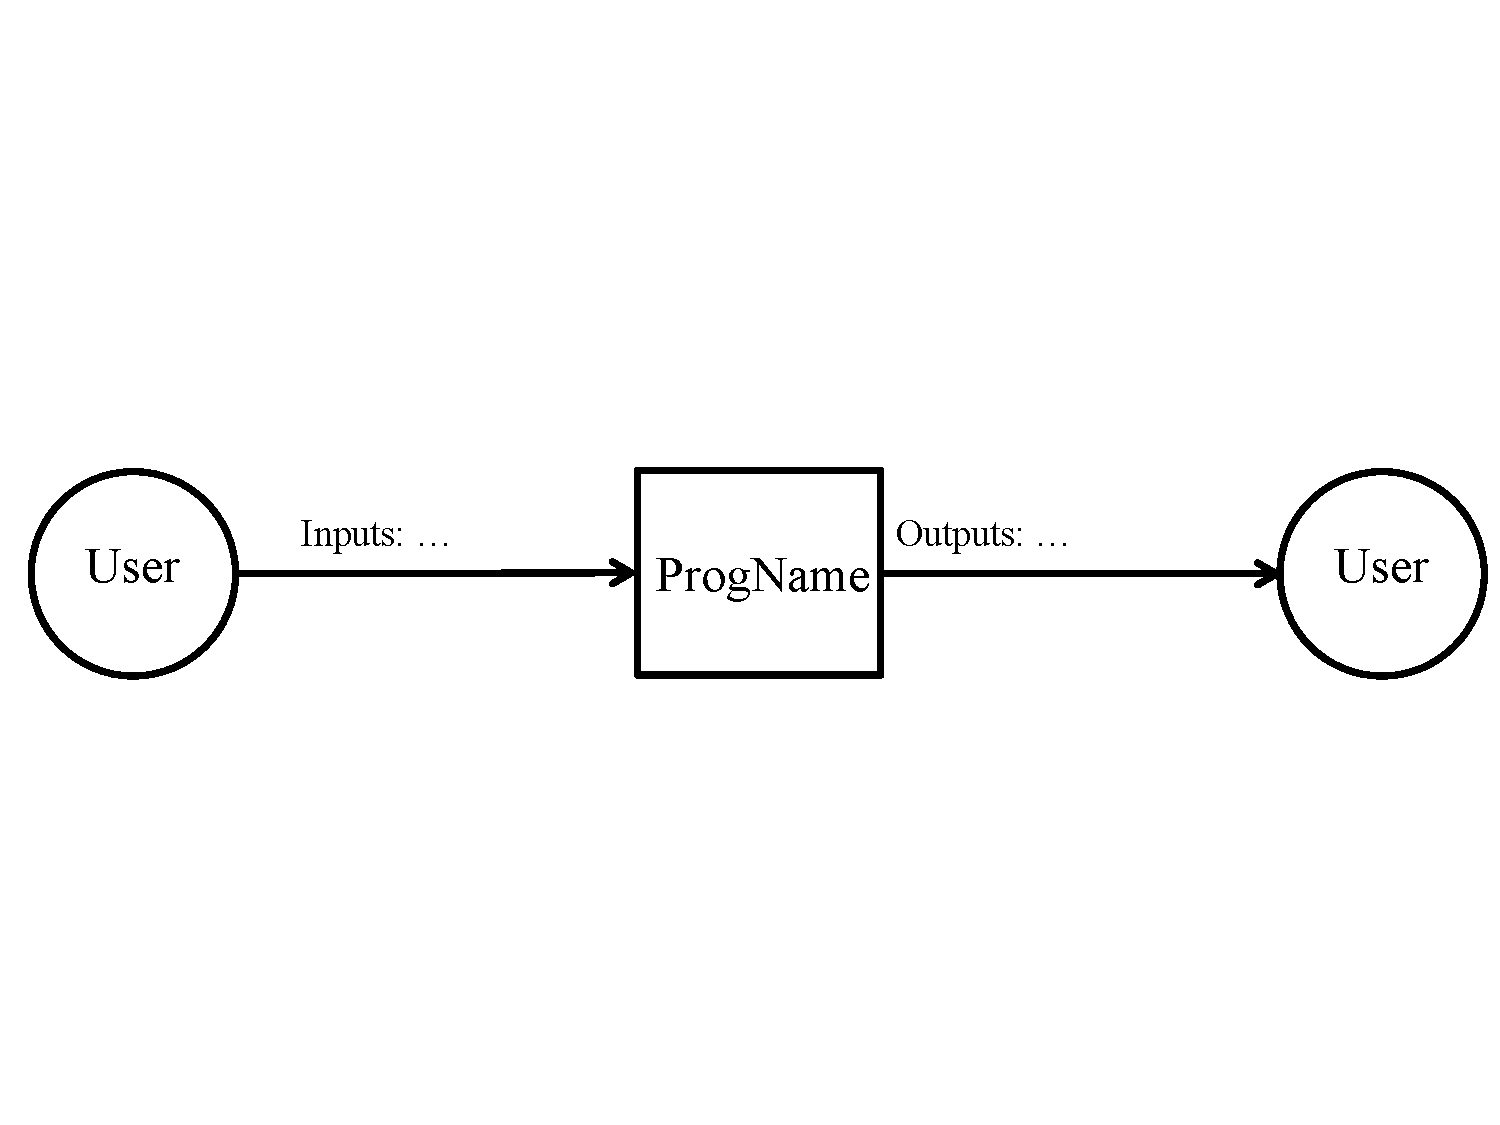
\includegraphics[width=0.6\textwidth]{SystemContextFigure}
\caption{System Context}
\label{Fig_SystemContext} 
\end{center}
\end{figure}

\plt{For each of the entities in the system context diagram its responsibilities
  should be listed.  Whenever possible the system should check for data quality,
  but for some cases the user will need to assume that responsibility.  The list
  of responsibilities should be about the inputs and outputs only, and they
  should be abstract.  Details should not be presented here.  However, the
  information should not be so abstract as to just say ``inputs'' and
  ``outputs''.  A summarizing phrase can be used to characterize the inputs.
  For instance, saying ``material properties'' provides some information, but it
  stays away from the detail of listing every required properties.}

\begin{itemize}
\item User Responsibilities:
\begin{itemize}
\item 
\end{itemize}
\item \progname{} Responsibilities:
\begin{itemize}
\item Detect data type mismatch, such as a string of characters instead of a
  floating point number
\item 
\end{itemize}
\end{itemize}

\plt{Identify in what context the software will typically be used.  Is it for
exploration? education? engineering work? scientific work?. Identify whether it
will be used for mission-critical or safety-critical applications.} \plt{This
additional context information is needed to determine how much effort should be
devoted to the rationale section.  If the application is safety-critical, the
bar is higher.  This is currently less structured, but analogous to, the idea to
the Automotive Safety Integrity Levels (ASILs) that McSCert uses in their
automotive hazard analyses.}

\wss{The }
\subsection{User Characteristics} \label{SecUserCharacteristics}

Users of the Damped Harmonic Oscillator software are expected to have a basic 
understanding of calculus and physics at an undergraduate level. Specifically, 
they should be familiar with the concepts of differential equations as they 
apply to motion and be able to apply basic physics principles to interpret 
the simulation results. This foundational knowledge is crucial for effective 
interaction with the software, enabling users to input realistic parameters 
and accurately interpret simulation outcomes.

\subsection{System Constraints}

Several key constraints influence the design and deployment of this software:

\begin{itemize}
  \item Platform Independence: It should run on common operating systems and 
  web browsers without special hardware requirements.
  \item Libraries and APIs: Where applicable, the software will rely on standard, 
  open-source libraries for mathematical computations and graphical displays 
  (e.g., NumPy, Matplotlib). The choice of these libraries is constrained by 
  their availability, documentation, and compatibility with the target operating 
  systems.
  \item User Interface: Aimed at users with a basic understanding of physics and 
  calculus, the software interface will prioritize simplicity to facilitate 
  learning and exploration without overwhelming users with unnecessary complexity.
\end{itemize}

\section{Specific System Description}

This section delves into the high-level overview of the problem that the Damped 
Harmonic Oscillator software aims to solve. Following this, the solution 
characteristics specification elaborates on the assumptions, theories, definitions, 
and instance models that explains the solution proposed by this project.

\subsection{Problem Description} \label{Sec_pd}

\progname{} targets the problem of accurately modeling and simulating the behavior 
of a damped harmonic oscillator. Such systems are essential in understanding 
phenomena where an object oscillates and gradually loses energy due to resistance 
or damping forces. This simulation is vital in fields such as mechanical 
engineering, where understanding the damping of oscillatory systems can lead to 
better designs and predictions.

\subsubsection{Terminology and  Definitions}

This subsection provides a list of terms that are used in the subsequent
sections and their meaning, with the purpose of reducing ambiguity and making 
it easier to correctly understand the requirements:

\begin{itemize}

\item \textbf{Isolated System:} Neglects external forces other than the damping 
and restoring forces.
\item \textbf{Harmonic Motion:} Assumes that in the absence of damping, the system 
would exhibit simple harmonic motion.
\item \textbf{Linear Damping:} A damping force that is directly proportional to 
the velocity of the oscillating object.
\item \textbf{Nonlinear Damping:} A damping force that varies with velocity in a 
non-proportional manner, often depending on the velocity's magnitude or other factors.

\end{itemize}

\subsubsection{Physical System Description} \label{sec_phySystDescrip}

The system comprises key elements crucial for its analysis and simulation:
\begin{itemize}
  \item \textbf{Mass (m):} Represents the inertia of the oscillating object.
  \item \textbf{Spring Constant (k):} Indicates the force needed to displace the 
  system from its equilibrium position.
  \item \textbf{Damping Coefficient (b):} For linear damping, quantifies the 
  proportionality between the damping force and velocity.
  \item \textbf{Damping Function (f(v)):} For nonlinear damping, represents the 
  relationship between damping force and velocity, which may vary based on the 
  system's specific characteristics.
\end{itemize}
 
 
The system's behavior is significantly influenced by the nature of the damping 
force. The model must account for both linear and nonlinear damping scenarios, 
with the interactions between the mass, spring constant, and damping forces 
defining the system's dynamic response.

% \plt{A figure here makes sense for most SRS documents}

% \begin{figure}[h!]
% \begin{center}
% %\rotatebox{-90}
% {
%  \includegraphics[width=0.5\textwidth]{<FigureName>}
% }
% \caption{\label{<Label>} <Caption>}
% \end{center}
% \end{figure}

\subsubsection{Goal Statements}

With the inclusion of both linear and nonlinear damping forces, the software aims 
to:

\begin{itemize}

  \item[GS\refstepcounter{goalnum}\thegoalnum \label{G_meaningfulLabel1}:] Create a simulation model that accurately represents the 
  behaviour of a damped harmonic oscillator in various scenarios.
  \item[GS\refstepcounter{goalnum}\thegoalnum \label{G_meaningfulLabel2}:] Facilitate the understanding of damping effects on 
  oscillatory systems through interactive and visual tools.
  \item[GS\refstepcounter{goalnum}\thegoalnum \label{G_meaningfulLabel3}:] Simulate of mathematical derivation.
  \item[GS\refstepcounter{goalnum}\thegoalnum \label{G_meaningfulLabel4}:] Design tools to allow users to create custom scenarios and 
  do comparative analysis. 
  \item[GS\refstepcounter{goalnum}\thegoalnum \label{G_meaningfulLabel5}:] Enhance educational understanding of damped oscillatory 
  systems.
  
\end{itemize}

\subsection{Solution Characteristics Specification}

This section elaborates on the mathematical and physical principles that form 
the basis of the solution, including assumptions, theoretical models, general 
definitions, and the derivation of instance models.

\subsubsection{Assumptions} \label{sec_assumpt}

This section simplifies the original problem and helps in developing the
theoretical model by filling in the missing information for the physical system.
The numbers given in the square brackets refer to the theoretical model [TM],
general definition [GD], data definition [DD], instance model [IM], or likely
change [LC], in which the respective assumption is used.

\begin{itemize}
\item[A\refstepcounter{assumpnum}\theassumpnum \label{A_meaningfulLabel}:]
\textbf{Constant Mass [TM, DD]:} The mass (m) of the oscillator is constant throughout the motion.
\item[A\refstepcounter{assumpnum}\theassumpnum \label{A_meaningfulLabel}:]
\textbf{Homogeneous Medium [TM, GD]:} Assumes the oscillator moves through a homogeneous medium, affecting the damping forces uniformly across the system.
\item[A\refstepcounter{assumpnum}\theassumpnum \label{A_meaningfulLabel}:]
\textbf{No External Forces [TM]:} External forces, other than damping and restoring forces, are neglected.
\item[A\refstepcounter{assumpnum}\theassumpnum \label{A_meaningfulLabel}:]
\textbf{Initial Conditions Known [IM]:} The initial position and velocity of the oscillator are known and specified.
\end{itemize}

\subsubsection{Theoretical Models}\label{sec_theoretical}

Theoretical models provide the mathematical foundation necessary for understanding and solving the dynamics of damped harmonic oscillators. These models incorporate physical laws and constitutive equations that describe how the system behaves under various conditions, including both linear and non-linear damping forces. The models are crucial for predicting system behavior and formulating solutions that can be applied in practical scenarios.

~\newline

\noindent
\deftheory
% #2 refname of theory
{TM:EOM-LDHO}
% #3 label
{Equation of Motion for Linearly Damped Harmonic Oscillators}
% #4 equation
{
  \begin{equation*}
    m*d\textsuperscript{2}x/dt\textsuperscript{2} + c*dx/dt + kx = 0
  \end{equation*}
}
% #5 description
{
  This equation models the motion of a damped harmonic oscillator, where $m$ is the mass of the oscillator, 
  $dx/dt$, $d\textsuperscript{2}x/dt\textsuperscript{2}$ represent the velocity and acceleration, respectively, 
  $c$ is the damping coefficient for linear damping, $k$ is the spring constant.
}
% #6 Notes
{
  None.
}
% #7 Source
{
  None
}
% #8 Referenced by
{
  None
}
% #9 Preconditions
{
  Assumes that the oscillator is subject to a restoring force proportional to displacement $x$ from equilibrium and a damping force that is linearly proportional to velocity.
}
% #1 derivation - not applicable by default
{}

\deftheory
% #2 refname of theory
{TM:EOM-NDHO}
% #3 label
{Equation of Motion for Non-Linearly Damped Harmonic Oscillators}
% #4 equation
{
  \begin{equation*}
    m*d\textsuperscript{2}x/dt\textsuperscript{2} + f(dx/dt) + kx = 0
  \end{equation*}
}
% #5 description
{
  This equation models the motion of a damped harmonic oscillator, where $m$ is the mass of the oscillator, 
  $dx/dt$, $d\textsuperscript{2}x/dt\textsuperscript{2}$ represent the velocity and acceleration, respectively, 
  $f(dx/dt)$ represents the function describing non-linear damping forces, $k$ is the spring constant.
}
% #6 Notes
{
  None.
}
% #7 Source
{
  None
}
% #8 Referenced by
{
  None
}
% #9 Preconditions
{
  Assumes that the oscillator is subject to a restoring force proportional to displacement $x$ from equilibrium and a damping force that follows non-linear relationship.
}
% #1 derivation - not applicable by default
{}

~\newline

\subsubsection{General Definitions}\label{sec_gendef}

This section collects the laws and equations that will be used in building the
instance models.

~\newline

\noindent
\begin{minipage}{\textwidth}
\renewcommand*{\arraystretch}{1.5}
\begin{tabular}{| p{\colAwidth} | p{\colBwidth}|}
\hline
\rowcolor[gray]{0.9}
Number& GD\refstepcounter{defnum}\thedefnum \label{NL}\\
\hline
Label &\bf Damping Force \\
\hline
% Units&$MLt^{-3}T^0$\\
% \hline
SI Units&\si{\newton}(Newton)\\
\hline
Equation& 
$ 
F\textsubscript{damping}=-c*dx/dt 
$ -- Linear Damping
\newline
$ 
F\textsubscript{damping}=-f(dx/dt)
$ -- Non-Linear Damping
\\
\hline
Description &
This definition differentiates between the damping forces in linear and 
non-linear systems. For linear systems, the force is proportional to the 
velocity$(dx/dt)$ with a constant$c$. In contrast, non-linear systems 
exhibit a damping force represented by $f(dx/dt)$, indicating a dependency 
on the velocity's magnitude or other factors.
\\
\hline
  Source & Hadley, Mark. "Damped Harmonic Oscillator" Department of Physics, Graz University of Technology \\
  \hline
  Ref.\ By & \ddref{IM1}, \ddref{DD1}\\
  \hline
\end{tabular}
\end{minipage}\\

~\newline

\noindent
\begin{minipage}{\textwidth}
\renewcommand*{\arraystretch}{1.5}
\begin{tabular}{| p{\colAwidth} | p{\colBwidth}|}
\hline
\rowcolor[gray]{0.9}
Number& GD\refstepcounter{defnum}\thedefnum \label{NL}\\
\hline
Label &\bf Natural Frequency of Oscillation \\
\hline
% Units&$MLt^{-3}T^0$\\
% \hline
SI Units&\si{\hertz}(Hertz)\\
\hline
Equation& 
$ 
\omega\textsubscript{0}=\sqrt{k/m} 
$
\\
\hline
Description &
This equation provides the natural frequency$(w\textsubscript{0})$ of an 
undamped harmonic oscillator, derived from the spring constant$(k)$ and 
mass$(m)$. It signifies the oscillator's inherent vibrational frequency 
absent damping forces.
\\
\hline
  Source & Hadley, Mark. "Damped Harmonic Oscillator" Department of Physics, Graz University of Technology \\
  \hline
  Ref.\ By & \ddref{IM1}, \ddref{DD3}, \ddref{DD4}\\
  \hline
\end{tabular}
\end{minipage}\\

~\newline

\noindent
\begin{minipage}{\textwidth}
\renewcommand*{\arraystretch}{1.5}
\begin{tabular}{| p{\colAwidth} | p{\colBwidth}|}
\hline
\rowcolor[gray]{0.9}
Number& GD\refstepcounter{defnum}\thedefnum \label{NL}\\
\hline
Label &\bf Energy Dissipation \\
\hline
% Units&$MLt^{-3}T^0$\\
% \hline
SI Units&\si{\joule}(Joules)\\
\hline
Equation& 
\textbf{Total Energy:} $ 
E=1/2*kx^{2}+1/2*mv^{2}
$
\newline
\textbf{Linear Damping Dissipation Rate:} $ 
dE/dt=-c*dx/dt
$
\newline
\textbf{Non-Linear Damping:} Energy Dissipation rate varies with $ 
f(dx/dt) 
$
\\
\hline
Description &
Outlines how the oscillator's total mechanical energy is influenced by 
damping. In linear damping scenarios, energy dissipation is directly 
proportional to the square of velocity, while in non-linear scenarios, 
it is dictated by a function of velocity, $f(dx/dt)$.
\\
\hline
  Source & Hadley, Mark. "Damped Harmonic Oscillator" Department of Physics, Graz University of Technology \\
  \hline
  Ref.\ By & \ddref{IM1}, \ddref{DD3}, \ddref{DD4}\\
  \hline
\end{tabular}
\end{minipage}\\

\subsubsection{Data Definitions}\label{sec_datadef}

This section collects and defines all the data needed to build the instance
models. The dimension of each quantity is also given.

~\newline

\noindent
\begin{minipage}{\textwidth}
\renewcommand*{\arraystretch}{1.5}
\begin{tabular}{| p{\colAwidth} | p{\colBwidth}|}
\hline
\rowcolor[gray]{0.9}
Number& DD\refstepcounter{datadefnum}\thedatadefnum \label{FluxCoil}\\
\hline
Label& \bf Damping Coefficient\\
\hline
Symbol & $c$ (linear damping), $f(dx/dt)$ (non-linear damping)\\
\hline
% Units& $Mt^{-3}$\\
% \hline
  SI Units & \si{\kilogram\per\second}\\
  \hline
  Equation& -\\
  \hline
  Description & 
  For linear damping, $c$ represents the constant proportionality factor 
  between the damping force and the velocity of the oscillator. For 
  non-linear damping, $f(dx/dt)$ represents a function defining the 
  relationship between the damping force and the velocity, which varies 
  with the velocity's magnitude or other system-specific factors.
  \\
  \hline
  Sources& "Damped Harmonic Oscillator" -- Wikipedia \\
  \hline
  Ref.\ By & \iref{ewat}\\
  \hline
\end{tabular}
\end{minipage}\\

~\newline

\noindent
\begin{minipage}{\textwidth}
\renewcommand*{\arraystretch}{1.5}
\begin{tabular}{| p{\colAwidth} | p{\colBwidth}|}
\hline
\rowcolor[gray]{0.9}
Number& DD\refstepcounter{datadefnum}\thedatadefnum \label{FluxCoil}\\
\hline
Label& \bf Mass\\
\hline
Symbol & $m$\\
\hline
% Units& $Mt^{-3}$\\
% \hline
  SI Units & \si{\kilogram}\\
  \hline
  Equation& -\\
  \hline
  Description & 
  Represents the mass of the harmonic oscillator. The mass is a crucial 
  parameter in determining the system's natural frequency and the dynamics 
  of its motion under damping forces.
  \\
  \hline
  Sources& "Damped Harmonic Oscillator" -- Wikipedia \\
  \hline
  Ref.\ By & \iref{GD2}\\
  \hline
\end{tabular}
\end{minipage}\\

~\newline

\noindent
\begin{minipage}{\textwidth}
\renewcommand*{\arraystretch}{1.5}
\begin{tabular}{| p{\colAwidth} | p{\colBwidth}|}
\hline
\rowcolor[gray]{0.9}
Number& DD\refstepcounter{datadefnum}\thedatadefnum \label{FluxCoil}\\
\hline
Label& \bf Spring Constant\\
\hline
Symbol & $k$\\
\hline
% Units& $Mt^{-3}$\\
% \hline
  SI Units & \si{\newton\per\metre}\\
  \hline
  Equation& -\\
  \hline
  Description & 
  The spring constant $k$ quantifies the stiffness of the spring in the 
  harmonic oscillator. It is a key factor in defining the natural 
  frequency of the oscillator and its response to applied forces.
  \\
  \hline
  Sources& "Damped Harmonic Oscillator" -- Wikipedia \\
  \hline
  Ref.\ By & \iref{GD2}\\
  \hline
\end{tabular}
\end{minipage}\\

~\newline

\noindent
\begin{minipage}{\textwidth}
\renewcommand*{\arraystretch}{1.5}
\begin{tabular}{| p{\colAwidth} | p{\colBwidth}|}
\hline
\rowcolor[gray]{0.9}
Number& DD\refstepcounter{datadefnum}\thedatadefnum \label{FluxCoil}\\
\hline
Label& \bf Natural Frequency\\
\hline
Symbol & $\omega_{0}$\\
\hline
% Units& $Mt^{-3}$\\
% \hline
  SI Units & \si{\radian\per\second}\\
  \hline
  Equation& -\\
  \hline
  Description & 
  The natural frequency $\omega_{0}$ of an undamped harmonic oscillator 
  is determined by its mass $m$ and spring constant $k$. This frequency 
  is foundational for analyzing the oscillator's behavior in the absence 
  of damping forces.
  \\
  \hline
  Sources& "Damped Harmonic Oscillator" -- Wikipedia \\
  \hline
  Ref.\ By & \iref{IM2}\\
  \hline
\end{tabular}
\end{minipage}\\

~\newline

\noindent
\begin{minipage}{\textwidth}
\renewcommand*{\arraystretch}{1.5}
\begin{tabular}{| p{\colAwidth} | p{\colBwidth}|}
\hline
\rowcolor[gray]{0.9}
Number& DD\refstepcounter{datadefnum}\thedatadefnum \label{FluxCoil}\\
\hline
Label& \bf Displacement\\
\hline
Symbol & $x$\\
\hline
% Units& $Mt^{-3}$\\
% \hline
  SI Units & \si{\metre}\\
  \hline
  Equation& -\\
  \hline
  Description & 
  Displacement $x$ from the equilibrium position provides a measure of 
  how far the oscillator moves over time. It is a fundamental quantity 
  for describing the oscillator's motion and is affected by both damping 
  forces and the system's natural dynamics.from the equilibrium position 
  provides a measure of how far the oscillator moves over time. It is a 
  fundamental quantity for describing the oscillator's motion and is 
  affected by both damping forces and the system's natural dynamics.
  \\
  \hline
  Sources& "Damped Harmonic Oscillator" -- Wikipedia \\
  \hline
  Ref.\ By & \iref{GD1}(Damping Force for Linear and Non-Linear Systems),
  \iref{IM1} (Displacement and Velocity Over Time)\\
  \hline
\end{tabular}
\end{minipage}\\

\subsubsection{Instance Models} \label{sec_instance}

This section transforms the problem defined in Section~\ref{Sec_pd} into 
one which is expressed in mathematical terms. It uses concrete symbols defined 
in Section~\ref{sec_datadef} to replace the abstract symbols in the models 
identified in Sections~\ref{sec_theoretical} and~\ref{sec_gendef}.

~\newline

%Instance Model 1

\noindent
\begin{minipage}{\textwidth}
\renewcommand*{\arraystretch}{1.5}
\begin{tabular}{| p{\colAwidth} | p{\colBwidth}|}
  \hline
  \rowcolor[gray]{0.9}
  Number& IM\refstepcounter{instnum}\theinstnum \label{ewat}\\
  \hline
  Label& \bf Equation of Motion\\
  \hline
  Input&Mass of the oscillator $m$, damping coefficient $c$ or $f(dx/dt)$, 
  spring constant $k$, initial displacement $x_{0}$, initial velocity $v_{0}$.\\
  \hline
  Output&Displacement $x{t}$ as a function of time $t$, Velocity $v(t)$ 
  as a function of time $t$.\\
  \hline
  Description&This model describes the motion of a damped harmonic oscillator by 
  incorporating linear or non-linear damping forces. The equation of motion 
  for linear damping is given by $m*d\textsuperscript{2}x/dt\textsuperscript{2} 
  + f(dx/dt) + kx = 0$, and for non-linear damping, it is modified to include a 
  non-linear damping term, represented by $f(dx/dt)$, affecting the velocity term.
  \\
  \hline
  Sources& Derived from the principles of mechanics as discussed in the provided 
  Wikipedia link and the Graz University of Technology's resource on damped 
  harmonic oscillators. \\
  \hline
  Ref.\ By & \iref{epcm}\\
  \hline
\end{tabular}
\end{minipage}\\

%~\newline

\subsubsection*{Derivation of Equation of Motion}

The equation is derived from Newton's second law of motion, $F=ma$, with force 
contributions from both the spring $(-kx)$ and the damping force ($-c*dx/dt$ 
or $-f(dx/dt)$). 

~\newline

%Instance Model 2

\noindent
\begin{minipage}{\textwidth}
\renewcommand*{\arraystretch}{1.5}
\begin{tabular}{| p{\colAwidth} | p{\colBwidth}|}
  \hline
  \rowcolor[gray]{0.9}
  Number& IM\refstepcounter{instnum}\theinstnum \label{ewat}\\
  \hline
  Label& \bf Energy Dissipation\\
  \hline
  Input&Spring constant $k$, mass $m$, damping coefficient $c$ or $f(dx/dt)$ 
  initial displacement $x_{0}$, initial velocity $v_{0}$.\\
  \hline
  Output&Total energy $E(t)$ of the system as a function of time $t$.\\
  \hline
  Description&This model quantifies the energy in the oscillator system and 
  its rate of dissipation due to damping. For linear damping, the rate of 
  energy dissipation is directly proportional to the square of the velocity, 
  whereas, for non-linear damping, the dissipation rate is a function of 
  velocity $f(dx/dt)$.
  \\
  \hline
  Sources& Based on energy conservation principles and the work-energy 
  theorem, adapted to include damping forces. \\
  \hline
  Ref.\ By & \iref{epcm}\\
  \hline
\end{tabular}
\end{minipage}\\

%~\newline

\subsubsection*{Derivation of Energy Dissipation}

The total mechanical energy $E(t)$ is given by the sum of kinetic and 
potential energy. The rate of change of this energy $(dE/dt)$ reflects energy 
dissipation due to damping.

\subsubsection{Input Data Constraints} \label{sec_DataConstraints}    

Table~\ref{TblInputVar} shows the data constraints on the input output
variables.  The column for physical constraints gives the physical limitations
on the range of values that can be taken by the variable.  The column for
software constraints restricts the range of inputs to reasonable values.  The
software constraints will be helpful in the design stage for picking suitable
algorithms.  The constraints are conservative, to give the user of the model the
flexibility to experiment with unusual situations.  The column of typical values
is intended to provide a feel for a common scenario.  The uncertainty column
provides an estimate of the confidence with which the physical quantities can be
measured.  This information would be part of the input if one were performing an
uncertainty quantification exercise.

The specification parameters in Table~\ref{TblInputVar} are listed in
Table~\ref{TblSpecParams}.

\begin{table}[!h]
  \caption{Input Variables} \label{TblInputVar}
  \renewcommand{\arraystretch}{1.2}
\noindent \begin{longtable*}{l l l l c} 
  \toprule
  \textbf{Var} & \textbf{Physical Constraints} & \textbf{Software Constraints} &
                             \textbf{Typical Value} & \textbf{Uncertainty}\\
  \midrule 
  $m$ & $m > 0$ & $m_{\text{min}} \leq m \leq m_{\text{max}}$ & 1
  \si[per-mode=symbol] {\kilogram} & 5\%\\

  $k$ & $k > 0$ & $k_{\text{min}} \leq k \leq k_{\text{max}}$ & 200 
  \si[per-mode=symbol] {\newton\per\meter} & 5\%\\

  $c$ & $c \geq 0$ & $c_{\text{min}} \leq c \leq c_{\text{max}}$ & 5 
  \si[per-mode=symbol] {\newton\second\per\meter} & 10\%\\

  $x_{0}$ & $x_{0} \geq 0$ & $x_{0_{min}} \leq x_{0} \leq 
  x_{0_{max}}$ & 0.1 \si[per-mode=symbol] {\meter} & 5\%\\

  $v_{0}$ & No constraint & $v_{0_{min}} \leq v_{0} \leq 
  v_{0_{max}}$ & 0 \si[per-mode=symbol] {\meter\per\second} & 5\%\\
  \bottomrule
\end{longtable*}
\end{table}

\noindent 
\begin{description}
\item[(*)] The software constraints are set to allow a wide range of scenarios, 
facilitating experimentation with both common and unusual situations. 
The specified typical values and uncertainties offer a baseline for standard 
simulations and uncertainty quantification exercises.
\end{description}

\begin{table}[h]
\caption{Specification Parameter Values} \label{TblSpecParams}
\renewcommand{\arraystretch}{1.2}
\noindent \begin{longtable*}{l l} 
  \toprule
  \textbf{Var} & \textbf{Value} \\
  \midrule 
  $m_\text{min}$ & 0.1 \si{\kilogram}\\
  $m_\text{max}$ & 10 \si{\kilogram}\\

  $k_\text{min}$ & 50 \si{\newton\per\meter}\\
  $k_\text{max}$ & 500 \si{\newton\per\meter}\\

  $c_\text{min}$ & 0 \si{\newton\second\per\metre}\\
  $c_\text{max}$ & 50 \si{\newton\second\per\metre}\\

  $x_{0_{min}}$ & 0 \si{\metre}\\
  $x_{0_{max}}$ & 1 \si{\metre}\\

  $v_{0_{min}}$ & -10 \si{\metre\per\second}\\
  $v_{0_{max}}$ & 10 \si{\metre\per\second}\\
  \bottomrule
\end{longtable*}
\end{table}

\newpage

\subsubsection{Properties of a Correct Solution} \label{sec_CorrectSolution}

\noindent
A correct solution must exhibit several fundamental physical principles and 
constraints. These criteria ensure that the model accurately reflects the 
behavior of real-world systems under both linear and non-linear damping 
forces. Below is an overview of these essential properties, along with a 
table summarizing the output variables and their physical constraints.

\subsubsection*{Essential Properties}

\begin{itemize}
  \item \textbf{Conservation of Energy (when applicable):} In the absence of external 
  forces, the total mechanical energy (kinetic plus potential) of the system 
  should be conserved over a complete cycle of motion in an undamped 
  oscillator. For damped oscillators, the solution must show a decrement in 
  total energy over time, corresponding to the energy dissipated due to damping.
  \item \textbf{Harmonic Motion:} The solution should exhibit characteristics of 
  harmonic motion, with periodicity and amplitude consistent with the input 
  parameters for the mass, spring constant, and damping coefficients.
  \item \textbf{Damping Behavior:} For linear damping, the solution must reflect an 
  exponential decay of motion amplitude over time. In the case of non-linear 
  damping, the solution should demonstrate amplitude decay behavior that 
  aligns with the non-linear damping force characteristics.
  \item \textbf{Equilibrium State:} The long-term behavior of the oscillator should 
  converge to a state of equilibrium, where the net force acting on the 
  oscillator is zero, especially under damping conditions.
  \item \textbf{Physical Realism:} The model's outputs must remain within physically 
  plausible ranges, considering the initial conditions and system parameters.
\end{itemize}

\begin{table}[!h]
\caption{Output Variables} \label{TblOutputVar}
\renewcommand{\arraystretch}{1.2}
\noindent \begin{longtable*}{l l} 
  \toprule
  \textbf{Var} & \textbf{Physical Constraints} \\
  \midrule 
  $x(t)$ & Must satisfy boundary conditions\\
  $v(t)$ & Consistent with $x(t)$ and damping\\
  $E(t)$ & Decreases over time for damped cases\\
  \bottomrule
\end{longtable*}
\end{table}

\section{Requirements}

\plt{The requirements refine the goal statement.  They will make heavy use of
  references to the instance models.}

This section provides the functional requirements, the business tasks that the
software is expected to complete, and the nonfunctional requirements, the
qualities that the software is expected to exhibit.

\subsection{Functional Requirements}

\noindent \begin{itemize}

\item[R\refstepcounter{reqnum}\thereqnum \label{R_Inputs}:] \plt{Requirements
    for the inputs that are supplied by the user.  This information has to be
    explicit.}

\item[R\refstepcounter{reqnum}\thereqnum \label{R_OutputInputs}:] \plt{It isn't
    always required, but often echoing the inputs as part of the output is a
    good idea.}

\item[R\refstepcounter{reqnum}\thereqnum \label{R_Calculate}:] \plt{Calculation
    related requirements.}

\item[R\refstepcounter{reqnum}\thereqnum \label{R_VerifyOutput}:]
  \plt{Verification related requirements.}

\item[R\refstepcounter{reqnum}\thereqnum \label{R_Output}:] \plt{Output related
    requirements.}

\end{itemize}

\plt{Every IM should map to at least one requirement, but not every requirement
  has to map to a corresponding IM.}

\subsection{Nonfunctional Requirements}

\plt{List your nonfunctional requirements.  You may consider using a fit
  criterion to make them verifiable.}
\plt{The goal is for the nonfunctional requirements to be unambiguous, abstract
  and verifiable.  This isn't easy to show succinctly, so a good strategy may be
to give a ``high level'' view of the requirement, but allow for the details to
be covered in the Verification and Validation document.}
\plt{An absolute requirement on a quality of the system is rarely needed.  For
  instance, an accuracy of 0.0101 \% is likely fine, even if the requirement is
  for 0.01 \% accuracy.  Therefore, the emphasis will often be more on
  describing now well the quality is achieved, through experimentation, and
  possibly theory, rather than meeting some bar that was defined a priori.}
\plt{You do not need an entry for correctness in your NFRs.  The purpose of the
  SRS is to record the requirements that need to be satisfied for correctness.
  Any statement of correctness would just be redundant. Rather than discuss
  correctness, you can characterize how far away from the correct (true)
  solution you are allowed to be.  This is discussed under accuracy.}

\noindent \begin{itemize}

\item[NFR\refstepcounter{nfrnum}\thenfrnum \label{NFR_Accuracy}:]
  \textbf{Accuracy} \plt{Characterize the accuracy by giving the context/use for
    the software.  Maybe something like, ``The accuracy of the computed
    solutions should meet the level needed for $<$engineering or scientific
    application$>$.  The level of accuracy achieved by \progname{} shall be
    described following the procedure given in Section~X of the Verification and
    Validation Plan.''  A link to the VnV plan would be a nice extra.}

\item[NFR\refstepcounter{nfrnum}\thenfrnum \label{NFR_Usability}:] \textbf{Usability}
  \plt{Characterize the usability by giving the context/use for the software.
    You should likely reference the user characteristics section.  The level of
    usability achieved by the software shall be described following the
    procedure given in Section~X of the Verification and Validation Plan.  A
    link to the VnV plan would be a nice extra.}

\item[NFR\refstepcounter{nfrnum}\thenfrnum \label{NFR_Maintainability}:]
  \textbf{Maintainability} \plt{The effort required to make any of the likely
    changes listed for \progname{} should be less than FRACTION of the original
    development time.  FRACTION is then a symbolic constant that can be defined
    at the end of the report.}

\item[NFR\refstepcounter{nfrnum}\thenfrnum \label{NFR_Portability}:]
  \textbf{Portability} \plt{This NFR is easier to write than the others.  The
    systems that \progname{} should run on should be listed here.  When possible
    the specific versions of the potential operating environments should be
    given.  To make the NFR verifiable a statement could be made that the tests
    from a given section of the VnV plan can be successfully run on all of the
    possible operating environments.}

\item Other NFRs that might be discussed include verifiability,
  understandability and reusability.

\end{itemize}

\subsection{Rationale}

\plt{Provide a rationale for the decisions made in the documentation.  Rationale
should be provided for scope decisions, modelling decisions, assumptions and
typical values.}

\section{Likely Changes}    

\noindent \begin{itemize}

\item[LC\refstepcounter{lcnum}\thelcnum\label{LC_meaningfulLabel}:] \plt{Give
    the likely changes, with a reference to the related assumption (aref), as appropriate.}

\end{itemize}

\section{Unlikely Changes}    

\noindent \begin{itemize}

\item[LC\refstepcounter{lcnum}\thelcnum\label{LC_meaningfulLabel}:] \plt{Give
    the unlikely changes.  The design can assume that the changes listed will
    not occur.}

\end{itemize}

\section{Traceability Matrices and Graphs}

The purpose of the traceability matrices is to provide easy references on what
has to be additionally modified if a certain component is changed.  Every time a
component is changed, the items in the column of that component that are marked
with an ``X'' may have to be modified as well.  Table~\ref{Table:trace} shows the
dependencies of theoretical models, general definitions, data definitions, and
instance models with each other. Table~\ref{Table:R_trace} shows the
dependencies of instance models, requirements, and data constraints on each
other. Table~\ref{Table:A_trace} shows the dependencies of theoretical models,
general definitions, data definitions, instance models, and likely changes on
the assumptions.

\plt{You will have to modify these tables for your problem.}

\plt{The traceability matrix is not generally symmetric.  If GD1 uses A1, that
  means that GD1's derivation or presentation requires invocation of A1.  A1
  does not use GD1.  A1 is ``used by'' GD1.}

\plt{The traceability matrix is challenging to maintain manually.  Please do
  your best.  In the future tools (like Drasil) will make this much easier.}

\afterpage{
\begin{landscape}
\begin{table}[h!]
\centering
\begin{tabular}{|c|c|c|c|c|c|c|c|c|c|c|c|c|c|c|c|c|c|c|c|}
\hline
	& \aref{A_OnlyThermalEnergy}& \aref{A_hcoeff}& \aref{A_mixed}& \aref{A_tpcm}& \aref{A_const_density}& \aref{A_const_C}& \aref{A_Newt_coil}& \aref{A_tcoil}& \aref{A_tlcoil}& \aref{A_Newt_pcm}& \aref{A_charge}& \aref{A_InitTemp}& \aref{A_OpRangePCM}& \aref{A_OpRange}& \aref{A_htank}& \aref{A_int_heat}& \aref{A_vpcm}& \aref{A_PCM_state}& \aref{A_Pressure} \\
\hline
\tref{T_COE}        & X& & & & & & & & & & & & & & & & & & \\ \hline
\tref{T_SHE}        & & & & & & & & & & & & & & & & & & & \\ \hline
\tref{T_LHE}        & & & & & & & & & & & & & & & & & & & \\ \hline
\dref{NL}           & & X& & & & & & & & & & & & & & & & & \\ \hline
\dref{ROCT}         & & & X& X& X& X& & & & & & & & & & & & & \\ \hline
\ddref{FluxCoil}    & & & & & & & X& X& X& & & & & & & & & & \\ \hline
\ddref{FluxPCM}     & & & X& X& & & & & & X& & & & & & & & & \\ \hline
\ddref{D_HOF}       & & & & & & & & & & & & & & & & & & & \\ \hline
\ddref{D_MF}        & & & & & & & & & & & & & & & & & & & \\ \hline
\iref{ewat}         & & & & & & & & & & & X& X& & X& X& X& & & X \\ \hline
\iref{epcm}         & & & & & & & & & & & & X& X& & & X& X& X& \\ \hline
\iref{I_HWAT}       & & & & & & & & & & & & & & X& & & & & X \\ \hline
\iref{I_HPCM}       & & & & & & & & & & & & & X& & & & & X & \\ \hline
\lcref{LC_tpcm}     & & & & X& & & & & & & & & & & & & & & \\ \hline
\lcref{LC_tcoil}    & & & & & & & & X& & & & & & & & & & & \\ \hline
\lcref{LC_tlcoil}   & & & & & & & & & X& & & & & & & & & & \\ \hline
\lcref{LC_charge}   & & & & & & & & & & & X& & & & & & & & \\ \hline
\lcref{LC_InitTemp} & & & & & & & & & & & & X& & & & & & & \\ \hline
\lcref{LC_htank}    & & & & & & & & & & & & & & & X& & & & \\
\hline
\end{tabular}
\caption{Traceability Matrix Showing the Connections Between Assumptions and Other Items}
\label{Table:A_trace}
\end{table}
\end{landscape}
}

\begin{table}[h!]
\centering
\begin{tabular}{|c|c|c|c|c|c|c|c|c|c|c|c|c|c|c|c|c|c|c|c|c|c|c|c|}
\hline        
	& \tref{T_COE}& \tref{T_SHE}& \tref{T_LHE}& \dref{NL}& \dref{ROCT} & \ddref{FluxCoil}& \ddref{FluxPCM} & \ddref{D_HOF}& \ddref{D_MF}& \iref{ewat}& \iref{epcm}& \iref{I_HWAT}& \iref{I_HPCM} \\
\hline
\tref{T_COE}     & & & & & & & & & & & & & \\ \hline
\tref{T_SHE}     & & & X& & & & & & & & & & \\ \hline
\tref{T_LHE}     & & & & & & & & & & & & & \\ \hline
\dref{NL}        & & & & & & & & & & & & & \\ \hline
\dref{ROCT}      & X& & & & & & & & & & & & \\ \hline
\ddref{FluxCoil} & & & & X& & & & & & & & & \\ \hline
\ddref{FluxPCM}  & & & & X& & & & & & & & & \\ \hline
\ddref{D_HOF}    & & & & & & & & & & & & & \\ \hline
\ddref{D_MF}     & & & & & & & & X& & & & & \\ \hline
\iref{ewat}      & & & & & X& X& X& & & & X& & \\ \hline
\iref{epcm}      & & & & & X& & X& & X& X& & & X \\ \hline
\iref{I_HWAT}    & & X& & & & & & & & & & & \\ \hline
\iref{I_HPCM}    & & X& X& & & & X& X& X& & X& & \\
\hline
\end{tabular}
\caption{Traceability Matrix Showing the Connections Between Items of Different Sections}
\label{Table:trace}
\end{table}

\begin{table}[h!]
\centering
\begin{tabular}{|c|c|c|c|c|c|c|c|}
\hline
	& \iref{ewat}& \iref{epcm}& \iref{I_HWAT}& \iref{I_HPCM}& \ref{sec_DataConstraints}& \rref{R_RawInputs}& \rref{R_MassInputs} \\
\hline
\iref{ewat}            & & X& & & & X& X \\ \hline
\iref{epcm}            & X& & & X& & X& X \\ \hline
\iref{I_HWAT}          & & & & & & X& X \\ \hline
\iref{I_HPCM}          & & X& & & & X& X \\ \hline
\rref{R_RawInputs}     & & & & & & & \\ \hline
\rref{R_MassInputs}    & & & & & & X& \\ \hline
\rref{R_CheckInputs}   & & & & & X& & \\ \hline
\rref{R_OutputInputs}  & X& X& & & & X& X \\ \hline
\rref{R_TempWater}     & X& & & & & & \\ \hline 
\rref{R_TempPCM}       & & X& & & & & \\ \hline
\rref{R_EnergyWater}   & & & X& & & & \\ \hline
\rref{R_EnergyPCM}     & & & & X& & & \\ \hline
\rref{R_VerifyOutput}  & & & X& X& & & \\ \hline
\rref{R_timeMeltBegin} & & X& & & & & \\ \hline
\rref{R_timeMeltEnd}   & & X& & & & & \\ 
\hline
\end{tabular}
\caption{Traceability Matrix Showing the Connections Between Requirements and Instance Models}
\label{Table:R_trace}
\end{table}

The purpose of the traceability graphs is also to provide easy references on
what has to be additionally modified if a certain component is changed.  The
arrows in the graphs represent dependencies. The component at the tail of an
arrow is depended on by the component at the head of that arrow. Therefore, if a
component is changed, the components that it points to should also be
changed. Figure~\ref{Fig_ATrace} shows the dependencies of theoretical models,
general definitions, data definitions, instance models, likely changes, and
assumptions on each other. Figure~\ref{Fig_RTrace} shows the dependencies of
instance models, requirements, and data constraints on each other.

% \begin{figure}[h!]
% 	\begin{center}
% 		%\rotatebox{-90}
% 		{
% 			\includegraphics[width=\textwidth]{ATrace.png}
% 		}
% 		\caption{\label{Fig_ATrace} Traceability Matrix Showing the Connections Between Items of Different Sections}
% 	\end{center}
% \end{figure}


% \begin{figure}[h!]
% 	\begin{center}
% 		%\rotatebox{-90}
% 		{
% 			\includegraphics[width=0.7\textwidth]{RTrace.png}
% 		}
% 		\caption{\label{Fig_RTrace} Traceability Matrix Showing the Connections Between Requirements, Instance Models, and Data Constraints}
% 	\end{center}
% \end{figure}

\section{Development Plan}

\plt{This section is optional.  It is used to explain the plan for developing
  the software.  In particular, this section gives a list of the order in which
  the requirements will be implemented.  In the context of a course  this is
  where you can indicate which requirements will be implemented as part of the
  course, and which will be ``faked'' as future work.  This section can be
  organized as a prioritized list of requirements, or it could should the
  requirements that will be implemented for ``phase 1'', ``phase 2'', etc.}

\section{Values of Auxiliary Constants}

\plt{Show the values of the symbolic parameters introduced in the report.}

\plt{The definition of the requirements will likely call for SYMBOLIC\_CONSTANTS.
Their values are defined in this section for easy maintenance.}

\plt{The value of FRACTION, for the Maintainability NFR would be given here.}

\newpage

\bibliographystyle {plainnat}
\bibliography {../../refs/References}

\newpage

\noindent \plt{The following is not part of the template, just some things to consider
  when filing in the template.}

\noindent \plt{Grammar, flow and \LaTeX advice:
\begin{itemize}
\item For Mac users \texttt{*.DS\_Store} should be in \texttt{.gitignore}
\item \LaTeX{} and formatting rules
\begin{itemize}
\item Variables are italic, everything else not, includes subscripts (link to
  document)
\begin{itemize}
\item \href{https://physics.nist.gov/cuu/pdf/typefaces.pdf}{Conventions}
\item Watch out for implied multiplication
\end{itemize}
\item Use BibTeX
\item Use cross-referencing
\end{itemize}
\item Grammar and writing rules
\begin{itemize}
\item Acronyms expanded on first usage (not just in table of acronyms)
\item ``In order to'' should be ``to''
\end{itemize}
\end{itemize}}

\noindent \plt{Advice on using the template:
\begin{itemize}
\item Difference between physical and software constraints
\item Properties of a correct solution means \emph{additional} properties, not
  a restating of the requirements (may be ``not applicable'' for your problem).
  If you have a table of output constraints, then these are properties of a
  correct solution.
\item Assumptions have to be invoked somewhere
\item ``Referenced by'' implies that there is an explicit reference
\item Think of traceability matrix, list of assumption invocations and list of
  reference by fields as automatically generatable
\item If you say the format of the output (plot, table etc), then your
  requirement could be more abstract
\end{itemize}
}

\newpage{}
\section*{Appendix --- Reflection}

The information in this section will be used to evaluate the team members on the
graduate attribute of Lifelong Learning.  Please answer the following questions:

\begin{enumerate}
  \item Which of the courses you have taken, or are currently taking, will help
  your team to be successful with your capstone project.
  \item What knowledge and skills will the team collectively need to acquire to
  successfully complete this capstone project?  Examples of possible knowledge
  to acquire include domain specific knowledge from the domain of your
  application, or software engineering knowledge, mechatronics knowledge or
  computer science knowledge.  Skills may be related to technology, or writing,
  or presentation, or team management, etc.  You should look to identify at
  least one item for each team member.
  \item For each of the knowledge areas and skills identified in the previous
  question, what are at least two approaches to acquiring the knowledge or
  mastering the skill?  Of the identified approaches, which will each team
  member pursue, and why did they make this choice?
\end{enumerate}

\end{document}